\documentclass[11pt]{article}
\usepackage[margin=0.82in]{geometry}
\usepackage{amsmath,amssymb,booktabs,tabularx,array,graphicx,caption,microtype,xcolor,hyperref,longtable}
\usepackage[T1]{fontenc}
\definecolor{linkblue}{HTML}{356AA0}
\hypersetup{colorlinks=true,linkcolor=linkblue,urlcolor=linkblue,citecolor=linkblue}
\newcommand{\orth}{\mathrm{ORTH}}
\newcommand{\plug}{\mathrm{PLUG}}
\newcommand{\riesz}{\mathrm{RIESZ}}
\newcommand{\R}{\mathbb{R}}
\newcommand{\E}{\mathbb{E}}
\newcommand{\pass}{\textcolor{linkblue}{\textbf{pass}}}
\newcommand{\fail}{\textcolor{orange}{\textbf{fail}}}
\newcolumntype{Y}{>{\raggedright\arraybackslash}X}
\newcommand{\EOneOrthNrmse}{0.104}
\newcommand{\EOneOrthCoverage}{0.940}
\newcommand{\EOneDirectMeanNrmse}{0.053}
\newcommand{\EOneDirectCovNrmse}{2.666}
\newcommand{\EFourDiscretePower}{1.000}
\newcommand{\EFourContinuousPower}{0.867}
\newcommand{\EFiveZeroNrmse}{0.016}
\newcommand{\ENineDirectAngle}{16.526}
\newcommand{\ENineCharAngle}{21.979}


\title{\textbf{Decisive Synthetic Validation of Predictive Distributional Jacobians}\\
\large What works, what fails, and what should be developed next}
\author{Local confirmatory study of the distributional SID runbook}
\date{July 14, 2026}

\begin{document}
\maketitle

\begin{abstract}
This report implements and tests the proposed cross-fitted Riesz-orthogonal estimator of derivatives of conditional future-feature expectations.  The program includes algebra and leakage gates, frozen development/confirmation separation, 30-seed confirmatory experiments for most synthetic claims, three nuisance initializations, exact oracle derivatives, direct typed baselines, and targeted failure tests.  A completion suite adds dependent trajectories with blocked/HAC inference, heteroskedastic noise and missingness, known/estimated/misspecified measurement correction, staged response-geometry stress tests, and a seven-family equal-access tournament against normalized mixture-density and spline-flow laws.  The result is neither a blanket success nor a failure.  The estimator is accurate and inferentially calibrated on regular synthetic problems, realizes the predicted second-order nuisance remainder, survives deterministic support motion, recovers history-local effects hidden by global cancellation, and detects moment-blind and path-order changes.  At the bounded local E10 budget, it is superior in the pooled seven-family comparison, but analytic MDNs have lower non-decisive mean errors in several individual cells.  Its present Riesz sieve fails under heavy tails and severe overlap; strong filtering and misspecified deconvolution block latent interpretation; and dense response geometry remains unresolved.  The defensible conclusion is therefore a restricted positive result for declared bounded predictive-feature projections, not a general neural-deployment claim.
\end{abstract}

\section{Executive decision}

\paragraph{Bottom line.}
The current approach is worth continuing, but only with a narrower claim and a different engineering priority.  The best-developed scientific object is the \emph{weak derivative of a declared bounded future-feature expectation}, estimated with cross-fitting and a history-side Riesz correction.  The strongest evidence is not that ORTH beats every baseline in point error.  It does not.  Its strongest evidence is that it combines reusable feature targets with calibrated uncertainty, remains meaningful when a likelihood score is singular, and resolves law/path changes that a fixed low-order target list cannot see.

\paragraph{What is already convincing.}
On the analytic Gaussian reference, ORTH characteristic-tangent NRMSE is \EOneOrthNrmse{} and coordinatewise coverage is \EOneOrthCoverage{}.  The controlled nuisance experiment matches the exact product-order bias prediction with $R^2>0.99999997$.  In the deterministic support limit, ORTH NRMSE is \EFiveZeroNrmse{} even though the likelihood history score is undefined.  With a frequency bank capable of resolving the alternatives, the moment-blind detection power is \EFourDiscretePower{} and \EFourContinuousPower{} in two distinct families.  A generic path bank detects event order in every confirmatory seed while endpoint and unordered summaries remain null.  In E10, every pooled analytic-MDN/NSF error ratio versus ORTH has a lower 95\% bound above the reciprocal superiority margin.

\paragraph{What is not convincing.}
ORTH has essentially the same point error as PLUG and RIESZ in regular cells; its paired E1 error ratio versus PLUG is $1.002$ with 95\% interval $[0.993,1.011]$.  The current Riesz sieve has zero empirical target coverage for Student-$t_3$ and low-density-gap separations 3--4.  Strong low-pass filtering ($\rho\ge .9$) makes the tested four-step effect essentially undetectable.  In the staged geometry suite, characteristic inversion has feature-tensor NRMSE 1.56--5.95 and response-subspace angles up to 78 degrees; direct or low-rank covariance heads are usually stronger, but source-subspace recovery remains poor for every method.  A known filter is recoverable at $\rho=.5$ (NRMSE 0.154) but not at $\rho=.98$ (NRMSE 1.002), and using $\rho=.5$ when truth is $.9$ drives coverage to 0.003.

\paragraph{Decision.}
Proceed with a paper/research claim about \emph{declared predictive-feature derivatives under diagnosed support and representation conditions}.  Do not treat the method as the default for known scalar targets, unknown dense covariance geometry, or filtered neural data.  Do not proceed to real-data interpretation until the Riesz and observation-process gates pass.

\begin{table}[t]
\centering
\footnotesize
\renewcommand{\arraystretch}{1.13}
\caption{Go/no-go summary.  ``Pass'' refers to the tested scope, not to unrestricted generality.}
\begin{tabularx}{\textwidth}{@{}p{0.55cm}p{3.35cm}p{2.45cm}Y@{}}
\toprule
ID & Question & Decision & Main consequence \\
\midrule
E0 & Algebra, software, and leakage & \pass & Core formulas, derivatives, splits, hashes, and boundary checks are operational. \\
E1 & Regular equal-access recovery & \pass, no point advantage & ORTH is useful for inference; direct mean remains better for a known mean target. \\
E2 & Practical orthogonality & \pass & The predicted second-order nuisance remainder is realized. \\
E3 & One future per history & \pass{} with HAC & Blocked estimates work through $\rho=.9$; IID standard errors under-cover. \\
E4 & Moment-blind law changes & \pass{} after amendment & Full-law value is real only at a declared resolving query bank. \\
E5 & Support motion/low noise & \pass & Weak features remain valid when likelihood scores diverge or disappear. \\
E6 & Riesz stability & \fail & No general observational-identification claim with the current sieve/diagnostic. \\
E7 & Heterogeneous cancellation & \pass{} at $R=2$ & Never interpret a zero global signed average as no local effect. \\
E8 & Observation process & \fail & Moderate correction works; severe filtering and misspecification block latent claims. \\
E9 & Dense unknown geometry & ORTH \fail & Prefer direct structured covariance heads at the tested scale. \\
E10 & Flexible law baselines & \pass{} pooled/local & ORTH wins pooled; no universal per-family winner and no scale frontier yet. \\
E11 & Path ordering & \pass & Supports future-path, rather than endpoint-only, feature claims. \\
\bottomrule
\end{tabularx}
\end{table}

\clearpage
\section{Estimator and implementation}

\subsection{The estimand}

For a history $H\in\R^{d_H}$, future path $Y^{[T]}$, and bounded feature map $\Phi_T$, define
\begin{align}
m_T(h) &= \E\{\Phi_T(Y^{[T]})\mid H=h\},\\
A_{r,p,T} &= \E\{b_r(H)\,\partial_{h_p}m_T(H)\}.
\end{align}
The target is a declared, history-weighted weak derivative.  It is not an unrestricted pointwise Jacobian, a causal effect, or a latent-state derivative.  Characteristic features are paired cosine/sine coordinates at a finite query bank.  Typed mean, covariance, moment, energy, and path-order readouts are treated as separate targets or controls.

For the linear functional $f\mapsto\E\{b_r(H)\partial_{h_p}f(H)\}$, a Riesz representer $\alpha_{r,p}$ satisfies
\begin{equation}
\E\{b_r(H)\partial_{h_p}f(H)\}=\E\{\alpha_{r,p}(H)f(H)\}.
\end{equation}
The orthogonal score is
\begin{equation}
\psi_{r,p,T}(O;m,\alpha)=
b_r(H)\partial_{h_p}m_T(H)
+\alpha_{r,p}(H)\{\Phi_T(Y^{[T]})-m_T(H)\}.
\end{equation}
All reported ORTH estimates average cross-fitted score contributions.  PLUG retains the first term only.  RIESZ uses $\alpha\Phi$.  OR-$M$, OR-$A$, and OR-$R$ oracle controls isolate the two nuisances.

\subsection{Concrete estimator}

The default conditional feature model is a differentiable random-feature sieve.  Fold-specific standardized histories feed an intercept, linear terms, centered quadratics, and 32 frozen $\tanh$ random features (64 for the largest dense cells).  Multivariate ridge regression predicts all feature coordinates jointly.  Its analytic derivative supplies $\partial_h\widehat m$.  The targeted Riesz coefficient is the ridge solution to the empirical Riesz loss in the same history sieve.  Fivefold cross-fitting keeps nuisance training outside the score fold.

This is intentionally a stable, inspectable first implementation rather than a large neural architecture.  The choice matters when interpreting failures: E6 is evidence against this nuisance approximation and diagnostic, not a theorem that no Riesz method can work.

\subsection{Baselines and controls}

The experimental tournament contains:
\begin{itemize}
\item ZERO, PLUG, RIESZ, and ORTH on the same feature bank;
\item oracle-nuisance decompositions OR-$M$, OR-$A$, and OR-$R$;
\item target-specific direct mean and symmetric covariance heads;
\item exact finite-moment null channels;
\item aligned motif controls for path ordering;
\item normalized MDNs with 5, 10, and 20 components and conditional rational-quadratic spline flows with 6 and 10 transforms in E10.
\end{itemize}
The E10 baselines expose exact normalized likelihoods and sampling-based characteristic expectations.  All methods share the same observational pairs, validation split, query bank, three initializations, and local training budget; internal sampling uses $B\in\{64,256,1024\}$.  This is the complete required reference-family grid at one deliberately bounded local sample/compute setting, not a large-scale compute Pareto frontier.

\section{Experimental governance and machine safety}

Development seeds were used for architecture/ridge selection; confirmatory seeds 1001--1030 were not touched until E2 passed.  Most central confirmatory families use 30 independent DGP seeds and three nuisance initializations.  The dependent E3 and measurement E8 extensions use 30 seeds and three initializations; staged E9 and neural E10 use ten seeds and three initializations because of their substantially larger per-cell cost.  Queries, configurations, environment locks, source snapshots, split assignments, checkpoints, seed-level CSV/Parquet files, and validation manifests are retained where implemented by the corresponding phase.

The local machine has 16 GiB memory and was deliberately run sequentially with one thread each for BLAS, OpenMP, and Torch, lowered process priority, a 10 GiB RSS ceiling, and a free-disk guard.  An early unchunked NSF development smoke reached 10.2 GiB and was stopped; chunking samples in batches of 32 reduced selected-run peak RSS to about 1.4 GiB.  No large models ran concurrently.  Reproducible score dumps and caches were removed under a written cleanup ledger, while all seed-level results and frozen provenance were retained.

\section{Core recovery and orthogonality: E0--E3}

\subsection{E0: implementation gates}

All ten algebra/software checks pass, and all fourteen package tests pass.  The analytic Gaussian characteristic derivative agrees with automatic differentiation to below $10^{-6}$; central differences show second-order convergence; exact Gaussian Riesz probes pass; an invalid uniform-boundary identity is rejected while a boundary-vanishing weight passes; oracle correction terms are centered; blocked/embargoed splits contain no footprint overlap; query banks and artifact hashes reproduce.

\subsection{E1: regular Gaussian recovery}

Figure~\ref{fig:e1} separates point recovery, inference, and typed baselines.  PLUG, RIESZ, and ORTH have nearly identical characteristic-tangent NRMSE near 0.104.  ORTH coverage is 0.940 and RIESZ coverage 0.975, whereas PLUG coverage is about 0.12 because it omits residual uncertainty.  The paired ORTH/PLUG error ratio is $1.002$ and the ORTH/RIESZ ratio $0.996$; neither satisfies the preregistered superiority rule.

The direct mean head is excellent (NRMSE \EOneDirectMeanNrmse{}), showing why direct regression remains the correct default for a known mean target.  The direct full covariance tensor is poor (NRMSE \EOneDirectCovNrmse{}), demonstrating that ``direct is best'' is not universal: the geometry and target dimension matter.

\begin{figure}[t]
\centering
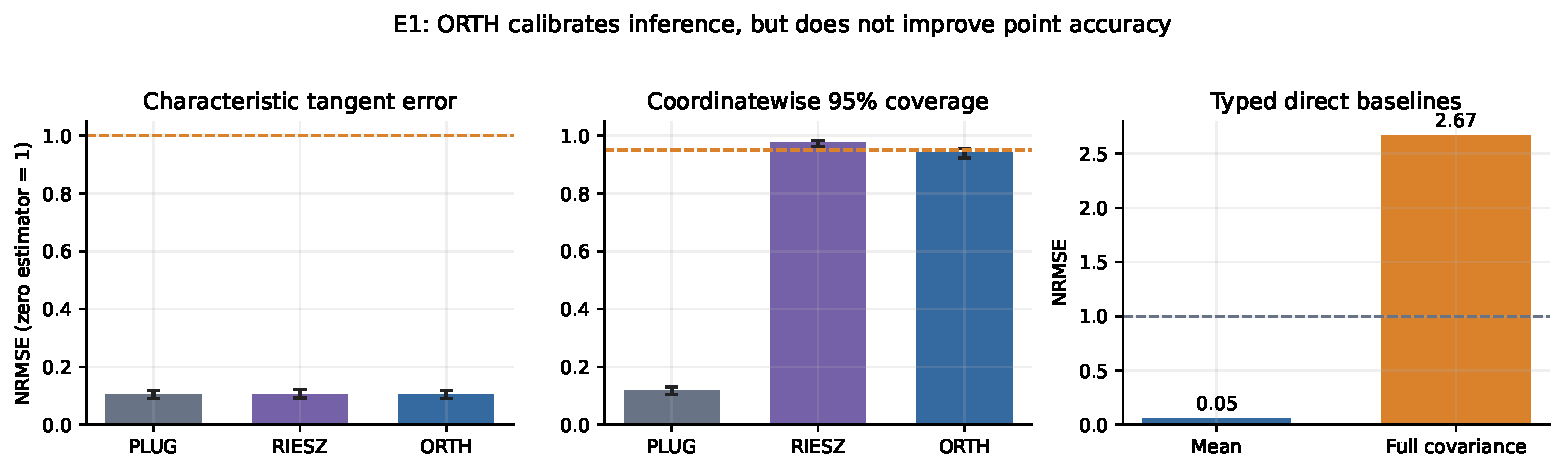
\includegraphics[width=\textwidth]{figures/e1_recovery.pdf}
\caption{E1 regular reference.  ORTH's benefit is calibrated inference, not lower point error.  Typed direct heads can be excellent or poor depending on target complexity.}
\label{fig:e1}
\end{figure}

\subsection{E2: the theory is visible in the data}

Artificial perturbations $\widehat m=m_0+a\delta_m$ and $\widehat\alpha=\alpha_0+b\delta_\alpha$ were applied after fixing the population law.  For linear, $\tanh$, and multivariate-$\tanh$ perturbations, ORTH bias is linear in the nuisance product $ab$ with fitted/theoretical slope relative error below $1.1\times10^{-4}$ and $R^2>0.99999997$.  Perturbing either nuisance alone leaves bias below $8.3\times10^{-6}$.  This is the cleanest positive evidence for the orthogonal score itself.

\subsection{E3: one future per high-dimensional history}

At $n=8{,}000$, IID ORTH NRMSE is 0.101 for $d_H=4$ and 0.111 for $d_H=16$.  At $d_H=32,n=32{,}000$ it is 0.070.  The dependent extension generates single AR(1) trajectories with $\rho\in\{.5,.9\}$ and stores observation-score rows.  With blocked folds, ORTH NRMSE is 0.107 at $d=16,\rho=.5$, 0.145 at $d=16,\rho=.9$, and 0.093 at $d=32,\rho=.9$; slopes are within 0.2\% of one.  Naive IID coverage falls to 0.881 and 0.836 in the two high-dependence cells, whereas HAC coverage is 0.949 and 0.951.  Random splitting is only modestly optimistic in point error, but does not repair invalid IID uncertainty.  The time-series claim is therefore supported only with blocked splitting and dependence-aware standard errors.

\begin{figure}[t]
\centering
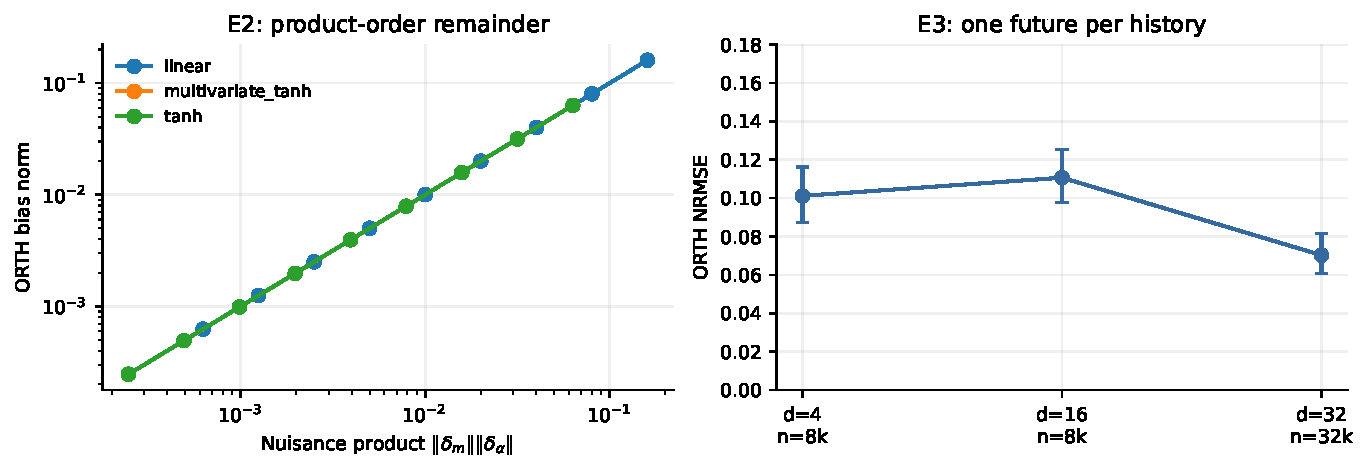
\includegraphics[width=0.92\textwidth]{figures/e2_e3_orthogonality_scaling.pdf}
\caption{E2 and E3.  The orthogonal remainder follows the nuisance-product prediction, and the estimator remains below the zero-error baseline with one future per continuous history.}
\end{figure}

\clearpage
\section{Distinctive law-level successes: E4, E5, E7, and E11}

\subsection{E4: moment-blind changes expose both the value and fragility of the feature bank}

Two DGPs change their conditional law while making the derivatives of the first four moments exactly zero: a smoothed finite-difference mixture and a continuous Legendre-$P_5$ tilt.  The original frequency bank $\{0.25,0.5,1,2\}$ failed badly (mean ORTH NRMSE 4.39).  On development seeds only, a frequency audit selected $\{1,2,4,8\}$, reducing mean NRMSE to 0.300.  This amendment was recorded before confirmation.

On 30 new seeds per family, characteristic power is 1.00 for the discrete family and 0.867 for the continuous family.  ORTH NRMSE is 0.168 and 0.412, with calibration slopes 1.009 and 1.019.  The first-four-moment FWER is 0.067 in both families (two calls in 30 seeds).  PLUG and RIESZ have similar point errors; again, orthogonalization is mainly inferential.

This is a real full-law advantage over a \emph{fixed finite moment list}.  It is not universal full-law recovery: a finite bank only sees the spectral region it queries.

\begin{figure}[t]
\centering
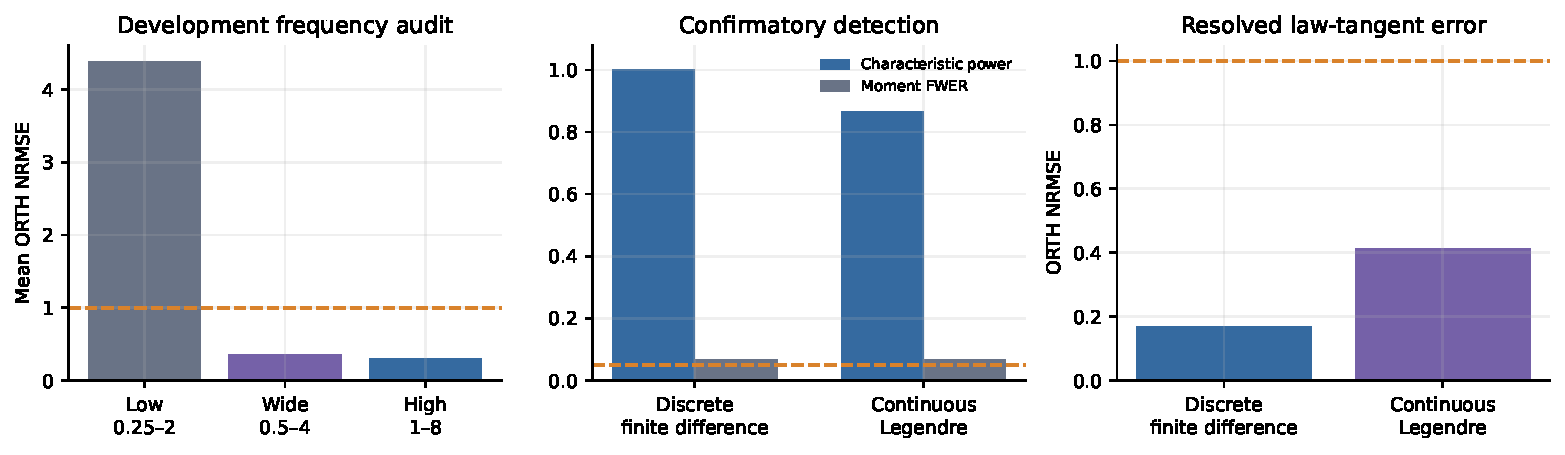
\includegraphics[width=\textwidth]{figures/e4_frequency_moment_blind.pdf}
\caption{E4.  The low-frequency bank is almost blind to the designed fifth-order alternatives.  A development-only spectral amendment resolves both families on confirmation.}
\end{figure}

\subsection{E5: weak features survive support motion}

For $Y=g(H)+\sigma\epsilon$, the noise ladder is $\sigma\in\{1,.3,.1,.03,.01,0\}$.  ORTH NRMSE improves from 0.018 at $\sigma=1$ to \EFiveZeroNrmse{} at $\sigma=0$; coverage stays near 0.95 and the calibration slope stays within 0.1\% of one.  In contrast, likelihood-score RMS grows from 1.16 to 116 as $\sigma$ drops from one to 0.01 and is undefined at zero.

This directly validates the theoretical reason for working with weak derivatives of bounded feature expectations: the predictive-law derivative can remain regular when a density score does not exist as an ordinary function.

\begin{figure}[t]
\centering
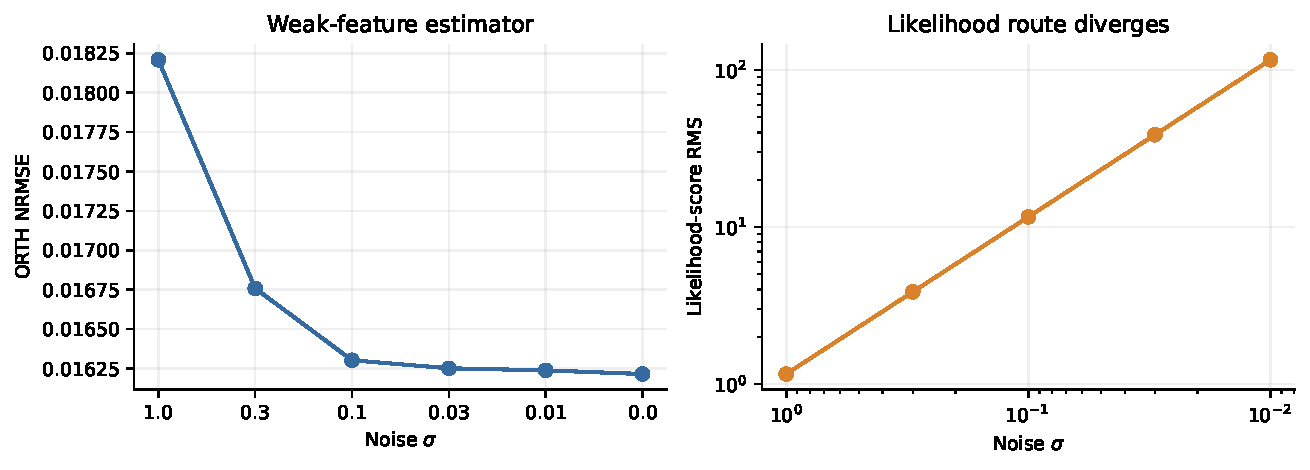
\includegraphics[width=0.88\textwidth]{figures/e5_support_motion.pdf}
\caption{E5.  The weak-feature target is stable through deterministic support; the likelihood-score route scales as $1/\sigma$ and disappears at zero noise.}
\end{figure}

\subsection{E7: a zero global average is not a null edge}

For $Y\mid H=h\sim N(h^2,\sigma^2)$, the derivative field $2h$ has zero global signed average but energy four.  The $R=1$ basis correctly estimates an average near zero.  The frozen $R=2$ Hermite basis recovers opposite signs in every seed, NRMSE 0.016, coverage 0.950, and projected energy 3.982 versus truth 4.000.  In the variance-cancellation family, $R=2$ NRMSE is 0.130, coverage 0.933, and energy 0.259 versus 0.262.  Moving to $R=4$ slightly improves approximation of the nonlinear field but reduces variance-family coverage to 0.869; higher resolution is not free.

\subsection{E11: path ordering is a second distinctive capability}

Forward and reverse event motifs have matched endpoints and unordered channel totals.  The generic full-path characteristic bank has ORTH NRMSE 0.209, slope 0.996, coverage 0.953, and power one.  Endpoint and unordered-total ORTH tests have FWER 0.056.  An aligned motif control is essentially exact.  PLUG calls the null summaries in every seed because its naive uncertainty ignores feature residuals, whereas ORTH controls them.

\begin{figure}[t]
\centering
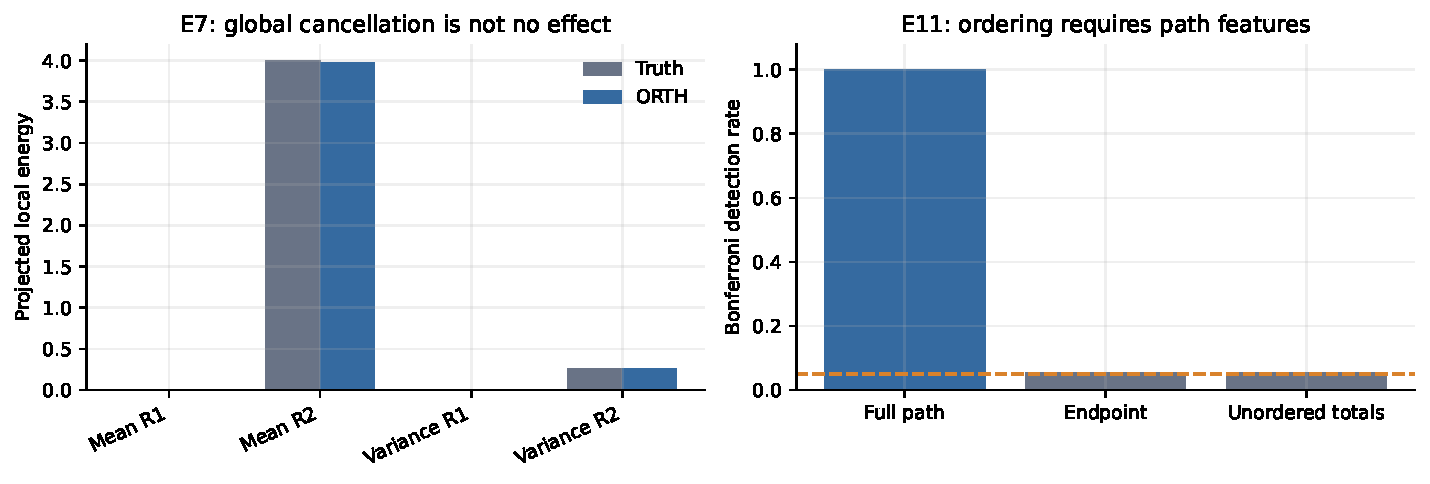
\includegraphics[width=0.94\textwidth]{figures/e7_e11_heterogeneity_path.pdf}
\caption{E7 and E11.  History resolution reveals cancellation, and path-aware features recover ordering invisible to endpoint/unordered summaries.}
\end{figure}

\clearpage
\section{The limiting gates: E6, E8, E9, and E10}

\subsection{E6: the present Riesz approximation is the main technical bottleneck}

The easy cases are good: Gaussian $\alpha$ NRMSE is 0.074; valid bounded-support weighting is 0.060; the $\operatorname{atanh}$ coordinate is 0.048; and the supported circle tangent is 0.075.  The implementation explicitly refuses the invalid $b=1$ uniform identity and a Euclidean radial perturbation that leaves the circle.

Heavy tails and weak overlap expose a failure.  Student-$t_{10}$ has NRMSE 0.138 and coverage 0.956, but $t_5$ coverage falls to 0.522 and $t_3$ to zero.  In the bridge-weighted Gaussian mixture, the oracle representer norm rises to 2.51 and 6.55 at separations three and four.  The fitted sieve instead collapses toward small norms, $\alpha$ NRMSE approaches one, and coverage is zero.  The warning rule catches all severe gap cells, but also fires too often in some easy cells; it is not well calibrated.

The theory predicts that identification depends on support, boundary behavior, and representer norm.  E6 is therefore not evidence that the theory is wrong.  It is evidence that a small unweighted random-feature sieve plus a fixed ridge is not an adequate general-purpose Riesz learner, and that the warning score needs its own null calibration.

\begin{figure}[t]
\centering
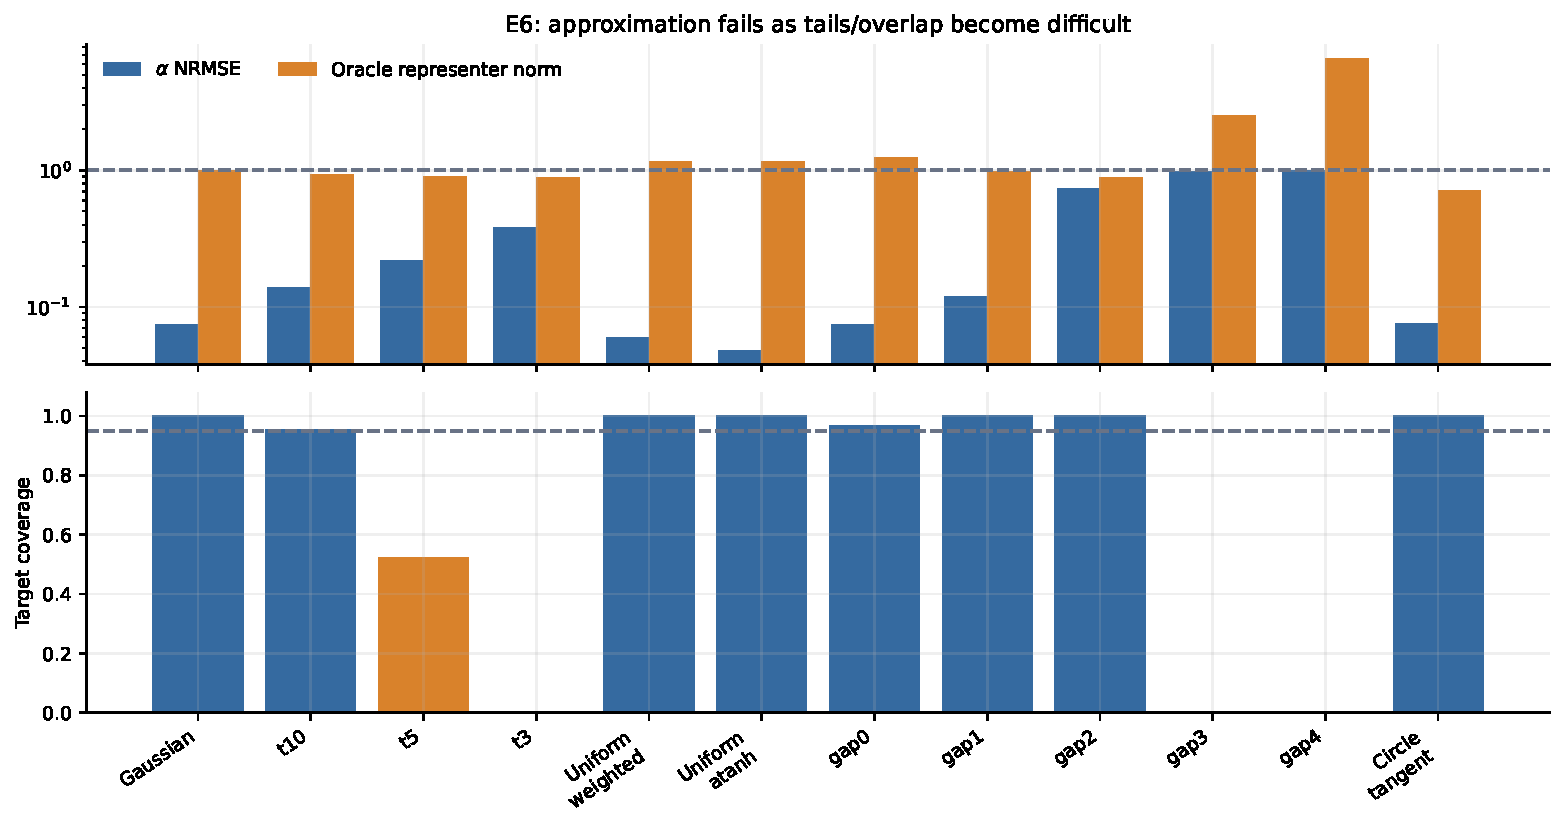
\includegraphics[width=\textwidth]{figures/e6_riesz_stability.pdf}
\caption{E6.  Easy interior and supported-direction cases work.  Heavy tails and bridge-weighted low-density gaps cause nuisance approximation and coverage failure.}
\end{figure}

\subsection{E8: observation-model failure blocks deployment}

The first observation suite contains a centered stochastic-gain path, filters $\rho\in\{0,.5,.9,.98\}$, 100 exact observed-law null seeds, and measurement-induced cross-talk.  Clean and $\rho=.5$ effects have power one.  With a four-step horizon, $\rho=.9$ and $.98$ attenuate the active impulse so strongly that the uncorrected observed-law target is essentially unavailable.  Cross-talk has power one and is correctly labeled an observed predictive effect rather than a latent biological effect.

The completion grid separates four issues.  First, heteroskedastic active cells remain calibrated: NRMSE is 0.262 and 0.168, slopes are 0.990 and 0.997, and coverage is 0.940--0.942.  A deliberately latent-null/observed-active heteroskedastic cell is detected in every seed, which is correct for the observed predictive claim and incorrect only if relabeled as a latent biological edge.  Second, supplying a history-dependent missingness mask improves NRMSE from 0.070 to 0.052; under harder MCAR deletion it improves 0.789 to 0.670, but the problem remains noisy.  Thus masks help without restoring lost information.

Third, known and jointly estimated one-parameter deconvolution agree.  At $\rho=.5$, NRMSE is 0.154--0.155 and estimated-$\rho$ error is 0.009.  At $\rho=.9$, NRMSE rises to 0.78--0.79 despite filter-estimation error below 0.02; at $\rho=.98$, NRMSE is approximately one and power is zero.  The dominant problem is ill-conditioning/information loss, not learning $\rho$.  Fourth, using $\rho=.5$ when truth is $.9$ gives NRMSE 0.926, slope 0.075, and coverage 0.003.  Measurement correction can therefore amplify model error.  E8 is complete and remains a hard no-go for latent real-data interpretation.

\subsection{E9: direct structure beats characteristic inversion for dense geometry}

The staged grid varies rank, rotations, source sparsity, history dimension, response dimension, and sample size.  In the easiest rank-one cells, direct covariance has NRMSE 0.49 and response-subspace angle 3.7--4.3 degrees; rank-selected low-rank projection reduces NRMSE to 0.23--0.25.  Characteristic inversion can recover the covariance tensor comparably in this easiest setting, but its native feature-tensor NRMSE remains 3.35--5.60.

The rank-three and higher-dimensional cells expose the limit.  In the axis-aligned rank-three cell, the direct response angle is 9.3 degrees but the source angle is 70.6 degrees; characteristic inversion has response/source angles 64.1/75.4 degrees.  At $n=32{,}000$, direct covariance NRMSE improves to 0.269 and characteristic feature NRMSE to 1.556, but source angles remain 58--66 degrees, and the low-rank selector obtains low tensor error by choosing an unstable response subspace.  With response dimension 32, direct NRMSE is 1.225 and characteristic inversion has feature NRMSE 5.953, response angle 78.3 degrees, and rank error 18.9.

This differs from E1, where the direct full covariance tensor failed.  The correct synthesis is conditional: a centered low-rank covariance DGP favors a typed covariance head, yet neither typed nor characteristic estimators reliably recover the unknown source geometry once multiple gains mix.  Characteristic features do not automatically solve the inverse readout problem, and E9 fails at the intended dense-geometry scope.

\begin{figure}[t]
\centering
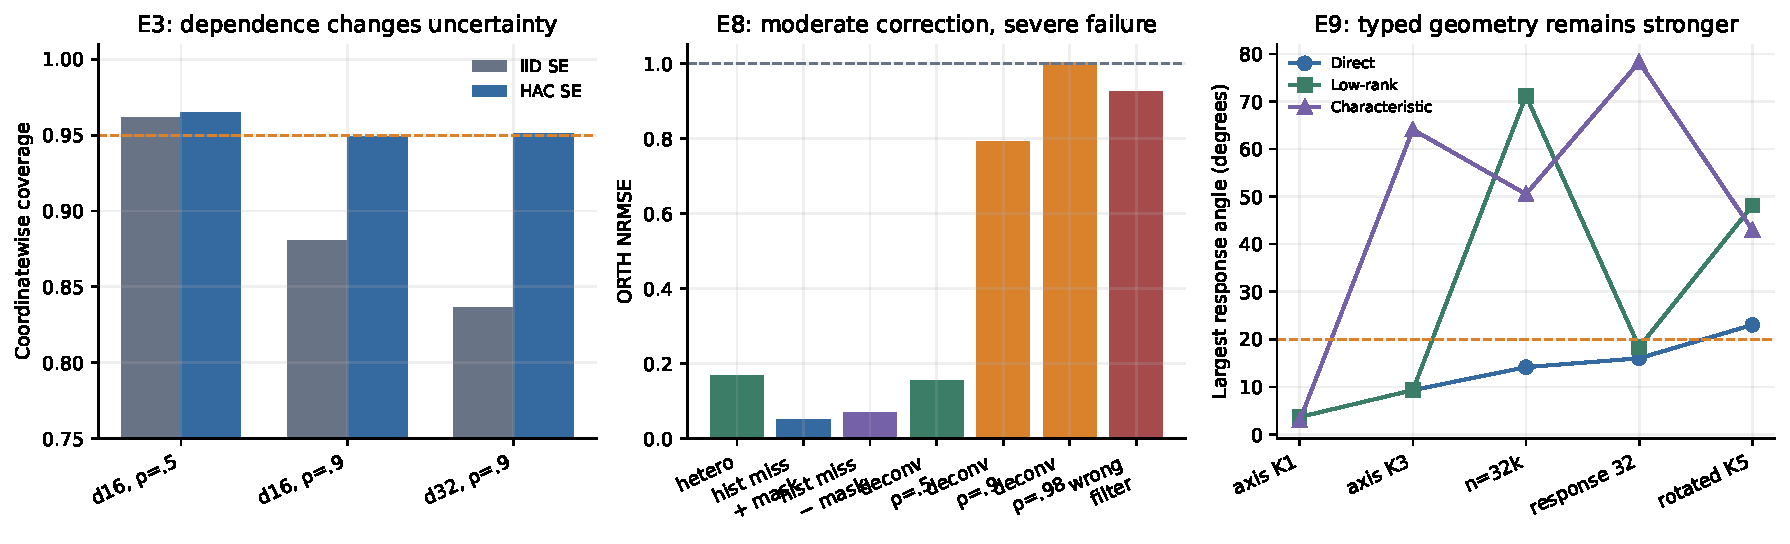
\includegraphics[width=\textwidth]{figures/completion_e3_e8_e9.pdf}
\caption{Completion suite.  Dependence-aware standard errors repair E3 coverage; E8 works for moderate observation problems but fails under severe or wrong deconvolution; typed covariance heads remain stronger in E9.}
\label{fig:completion_gates}
\end{figure}

\subsection{E10: a pooled local-budget win, not universal dominance}

The completed local tournament uses all seven required reference families, $n=4{,}000$, ten DGP seeds, three initializations, and at most ten training epochs.  Primary reusable-law comparators are full-covariance MDNs with $K\in\{5,10,20\}$ and exact analytic characteristic/autodiff readout, plus normalized rational-quadratic spline flows with 6 and 10 transforms evaluated at $B=1024$.  A second autoregressive MDN readout and all neural methods are also evaluated by common-random-number sampling at $B\in\{64,256,1024\}$.  All fits succeed and characteristic-modulus checks pass.

\begin{table}[t]
\centering
\footnotesize
\caption{E10 mean tangent NRMSE.  Bold is the lowest mean in a row; it is not automatically a statistically superior method.  MDN-A denotes the analytic full-covariance mixture readout.}
\begin{tabular}{@{}lrrrrrr@{}}
\toprule
Family & ORTH & MDN-A5 & MDN-A10 & MDN-A20 & NSF-6 & NSF-10 \\
\midrule
E1 Gaussian & 0.160 & \textbf{0.150} & 0.151 & 0.163 & 0.179 & 0.178 \\
E4 discrete & \textbf{0.235} & 1.082 & 1.063 & 1.057 & 0.431 & 0.413 \\
E4 continuous & \textbf{0.707} & 1.197 & 1.082 & 0.939 & 1.115 & 1.223 \\
E5 support motion & 0.021 & 0.028 & 0.023 & \textbf{0.018} & 0.030 & 0.033 \\
E8 filtered & \textbf{0.688} & 1.050 & 1.097 & 1.074 & 1.126 & 1.216 \\
E9 dense & 6.280 & 6.317 & 4.920 & \textbf{3.890} & 10.015 & 10.160 \\
E11 ordering & \textbf{0.279} & 0.914 & 0.956 & 0.968 & 0.789 & 0.719 \\
\bottomrule
\end{tabular}

\label{tab:e10_primary}
\end{table}

ORTH has the lowest mean in the two moment-blind families, the filtered family, and path ordering.  Analytic MDNs have slightly lower means in E1 and E5 and a larger apparent advantage in E9; none of those MDN/ORTH comparisons clears the preregistered requirement that the upper 95\% error-ratio bound be below 0.90.  Conversely, ORTH is superior to every MDN and NSF in E4-discrete, E4-continuous, E8, and E11.  In E9, ORTH beats both NSFs but not the analytic MDNs.  Across all seven paired families, neural/ORTH geometric error ratios are 1.57--1.77 and every pooled interval declares ORTH superior.

The relative ranking must not erase absolute failure.  E8 ORTH NRMSE is 0.688 and E9 ORTH NRMSE is 6.280; the best E9 analytic MDN is still 3.890.  Neither measurement nor dense-geometry gate passes.  Internal sampling is also scientifically material: at $B=64$, autoregressive-MDN error is 2.25--3.09 times its $B=1024$ error, whereas NSF inflation is 1.10--1.14.  Replacing sampled MDN tangents with the exact analytic readout changes several mean rankings, demonstrating that derivative/readout design is part of the baseline, not a harmless implementation detail.

\begin{figure}[t]
\centering
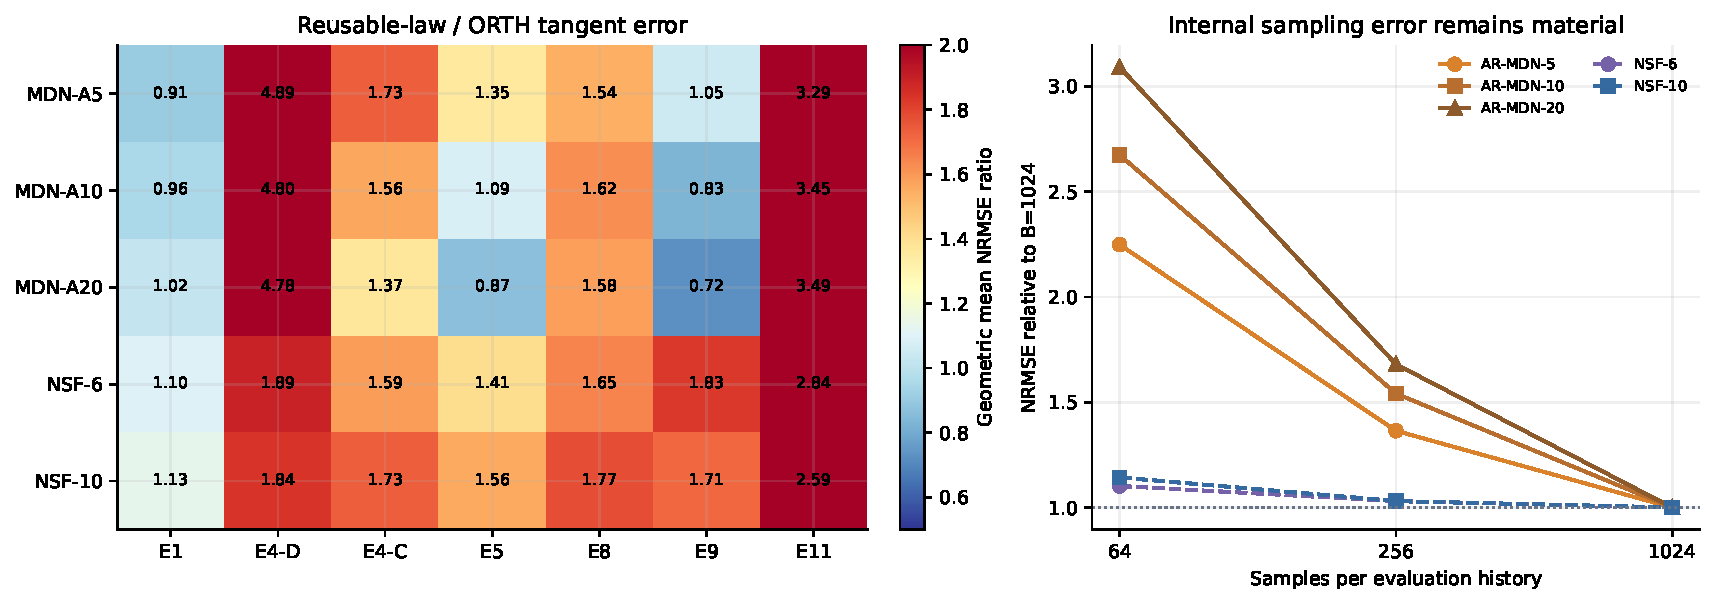
\includegraphics[width=\textwidth]{figures/e10_full_tournament.pdf}
\caption{E10.  Left: paired reusable-law/ORTH tangent-error ratios by family; values below one favor the reusable law.  Right: sampling-based tangent error relative to $B=1024$.  The pooled ORTH advantage coexists with inconclusive or reversed mean rankings in E1, E5, and E9.}
\label{fig:e10_full}
\end{figure}

\clearpage
\section{What is wrong: theory, synthetic model, or implementation?}

The experiments separate four different failure modes.

\subsection{The core orthogonal-score theory is not the main problem}

E0 and E2 directly validate the algebra and second-order remainder.  E5 validates the weak-feature motivation in a case where likelihood scores become ill-conditioned.  These are difficult results to explain as accidental simulator matching.  The basic estimand and score are sound in the tested regularity class.

\subsection{Representation is a scientific design choice}

The first E4 bank failed because its frequencies were too low to resolve a fifth-order spectral departure.  No estimator can recover a feature direction that the declared representation barely sees.  Query-bank resolution must therefore be treated like measurement resolution: frozen, audited on development data, and reported as part of the claim.  Multi-scale banks, held-out witness stability, and explicit spectral power curves are more important than enlarging a response-score model.

\subsection{The Riesz nuisance and its diagnostic are underdeveloped}

E6 is the largest obstacle to a general claim.  The fixed sieve/ridge works in regular interiors and fails under tail/overlap stress.  The representer can concentrate where histories are rare, exactly where unweighted regression is least reliable.  A useful system must distinguish (i) estimable but hard, (ii) estimable only after changing the weight/trimmed estimand, and (iii) unsupported directions.  The current code handles obvious boundary/manifold refusals but not the first two reliably.

\subsection{Some synthetic cells reveal genuine information limits}

The $\rho=.98$ observation cell is not primarily an optimizer failure.  A four-step low-pass kernel carries very little of the current latent shock.  The correct remedy is longer horizons, a declared measurement model, or deconvolution---not forcing the same estimator to report a large effect.  Likewise, dense covariance recovery is a high-dimensional inverse problem; a generic feature tensor and a typed low-rank head expose different information and inductive biases.

\subsection{The baseline suite supports a bounded ranking, not a global one}

Direct mean regression is decisively strong for known mean effects.  Direct covariance is strong in E9 and weak in E1.  E10 now supports a paired ranking at one local sample/compute budget: ORTH wins in aggregate and in the feature-resolution/path families, while analytic MDNs have lower but non-decisive mean errors in several smooth or dense cells.  The method choice remains task-dependent:
\begin{itemize}
\item known low-dimensional typed target: calibrated direct head;
\item many bounded queries plus valid Riesz diagnostics: ORTH feature estimator;
\item dense structured covariance: typed low-rank covariance head;
\item high-quality generation or arbitrary downstream queries: flexible normalized law, if its tangent is validated;
\item finite intervention contrast: finite-contrast estimator rather than an observational derivative.
\end{itemize}

\section{Recommended next program}

\subsection*{Priority 1: rebuild and calibrate the Riesz layer}

Compare targeted sieves, density-score/Stein estimators, RKHS representers, and weighted neural Riesz objectives on E6.  Train explicitly on tail/bridge probes; use regularization paths; estimate effective representer norms on held-out histories; and calibrate warning thresholds on at least 100 green and 100 invalid/unstable seeds.  When trimming or bridge weighting changes the estimand, record the new $b(H)$ and do not present it as the original target.

\subsection*{Priority 2: map measurement identifiability, not another matched correction}

E8 now includes heteroskedastic noise, missingness with/without masks, known and estimated one-parameter deconvolution, and misspecification.  The next work should vary horizon with filter condition number, use partial-identification bounds when high-frequency information is lost, and stress richer observation models outside the fitted family.  Every result must report observed-law and latent-law targets separately.  The aim is to discover when latent recovery is possible, not to force a corrected point estimate in every cell.

\subsection*{Priority 3: turn E10 into a sample/compute frontier}

The required seven-family local grid is complete.  Next vary $n$, optimizer steps, model width/depth, and evaluation-history count while preserving the analytic MDN readout and $B\in\{64,256,1024\}$ for non-analytic laws.  Add reparameterized derivative estimators and a stabilized score/diffusion or flow-matching generator as a separate generative comparison.  Report likelihood/energy score and tangent NRMSE separately.  The key question is whether flexible laws close the tangent gap with scale or whether the targeted estimator retains a statistical/compute advantage.

\subsection*{Priority 4: preserve distinctive features without overclaiming}

For E4, use a predeclared multi-scale bank and report resolution curves.  For E11, add the permutation-motif family, signature-kernel features, time jitter/noise sweeps, and path-witness stability across seeds.  These experiments are currently the clearest reason to prefer a reusable feature representation over a finite list of typed heads.

\subsection*{Priority 5: extend dependence beyond the E3 reference}

Blocked folds, HAC uncertainty, and retained observation-score rows now pass in the dependent E3 reference.  Repeat the same discipline for heterogeneous E7 and path-order E11 trajectories, add embargo sensitivity, and compare HAC with a trajectory/block multiplier bootstrap.  IID standard errors must not be reported for overlapping or highly persistent histories.

\section{Reproducibility and artifact map}

The implementation lives under \path{distributional_sid/}, with core, extension, and remaining-experiment modules in \path{src/distributional_sid/}.  Frozen run directories are under \path{distributional_sid/runs/}.  Each selected run contains a machine-readable summary and validation file; earlier failed packaging attempts are retained with suffixes and excluded from this report.  Disk removals are documented in \path{CLEANUP_20260714.md}.

This report is regenerated by \path{reports/distributional_sid_decisive_2026-07-14/make_report.py}.  The machine-readable decision record is \path{results_snapshot.json}.  Full claim and artifact registries are \path{tables/claim_registry.csv}, \path{tables/gate_matrix.csv}, and \path{tables/artifact_ledger.csv}.  The report uses only final selected run directories, whose summary hashes are stored in the ledger.

\section{Final conclusion}

The project now has a coherent empirical answer.  The most developed idea is not ``estimate a response score and manipulate it into a SID,'' nor ``learn an unrestricted full law.''  It is:
\begin{quote}
Estimate declared, history-weighted derivatives of bounded predictive future features with cross-fitting and an explicit Riesz identification layer; use the feature bank to choose what aspects of the law are visible, and refuse claims when support, overlap, measurement, or readout diagnostics fail.
\end{quote}
That object works convincingly in regular synthetic settings and has two distinctive successes---moment-blind law changes and path ordering---plus a strong support-motion result.  ORTH's practical advantage is calibrated inference, nuisance robustness, and efficient targeting of a declared derivative; it is not uniformly lower point error in easy smooth cells.  The normalized-law tournament now suggests a real local-budget advantage overall, while also showing that exact analytic readouts can reverse family-level mean rankings.  The next advances must come from Riesz stability, measurement identifiability, and a sample/compute frontier for reusable laws.  More experiments on the same easy matched simulator would add little.

\end{document}
